\documentclass[11pt,bibliography=totocnumbered]{article}
\usepackage{amsmath, amssymb, amsthm}
\usepackage{bm, bbm}
\usepackage{booktabs}
\usepackage{enumerate}
\usepackage{fancyhdr}
\usepackage[margin=1in]{geometry}
\newcommand{\HRule}{\rule{\linewidth}{0.5mm}} 
\usepackage[hidelinks]{hyperref}
\usepackage{float}
\hypersetup{
	colorlinks=true,
	linkcolor=blue,
	filecolor=magenta,      
	urlcolor=cyan,
}
\usepackage{lastpage}
\usepackage{svg}
\usepackage{tikz}
\usepackage{pgfplots}
\usepackage{siunitx}
\usepgfplotslibrary{groupplots}
\usepackage{listings} 
\usepackage{color}
\lstset{
	numbers=left, 
	numberstyle= \tiny, 
	keywordstyle= \color{blue!98},
	commentstyle= \color{red!50!green!50!blue!50}, 
	frame=shadowbox, 
	rulesepcolor= \color{ red!20!green!20!blue!20} ,
	escapeinside=``, 
	xleftmargin=1.5em,xrightmargin=1.5em, aboveskip=0.5em,
	framexleftmargin=1.5em,
	basicstyle=\footnotesize\ttfamily
} 
\usepackage{enumitem} 
\makeatletter
\let\@afterindentfalse\@afterindenttrue
\@afterindenttrue
\makeatother
\setlength{\parindent}{2em}

\pagestyle{fancy}
\lhead{\textsc{CSC4001, Proposal}}
\chead{\today}
\rhead{Medical Bot}

\newcommand{\mtx}[1]{\mathbf{#1}}
\renewcommand{\vec}[1]{\mathbf{#1}}
\DeclareMathOperator{\reals}{\mathbb{R}}
\DeclareMathOperator{\diag}{diag}
\newcommand{\abs}[1]{\left|{#1}\right|}
\newcommand{\tabincell}[2]{\begin{tabular}{@{}#1@{}}#2\end{tabular}}

\begin{document}
  \begin{titlepage}
  	
  	\begin{center}
  		
  		% Upper part of the page
  		
\includegraphics[width=0.35\textwidth]{./figures/logo.png}\\[0.5cm]    
  		
  		\textsc{\Large The Chinese University of Hong Kong, Shenzhen}\\[1.5cm]
  		
  		\textsc{\large CSC4001 Project Proposal}\\[0.5cm]
  		
  		% Title
  		\HRule \\[0.6cm]
  		{ \huge \bfseries Web-based Medical Bot}\\[0.4cm]
  		
  		\HRule \\[1.5cm]
  		
  		% Author and IDs
  		\begin{minipage}{0.4\textwidth}
  			\begin{flushleft} \large
  				\emph{Authors:}\\[0.5cm]
  				\textsc{Chen} Yaqian\\[0.5cm]
  				\textsc{Liu} Jiazhen\\[0.5cm]
  				\textsc{Xiao} Shiting\\[0.5cm]
  				\textsc{Xue} Chunyue \\[0.5cm]
  				\textsc{Zhou} Zheyuan\\[0.5cm]
  			\end{flushleft}
  		\end{minipage}
  		\begin{minipage}{0.4\textwidth}
  			\begin{flushright} \large
  				\emph{Student IDs:} \\[0.5cm]
  				117010032\\[0.5cm]
  				117010168\\[0.5cm]
  				116010243\\[0.5cm]
  				116010255\\[0.5cm]
  				117010423\\[0.5cm]
  			\end{flushright}
  		\end{minipage}
  		\vfill
  		
  		% Bottom of the page
  		{\large \today}
  		
  	\end{center}
  	
  \end{titlepage}

	\tableofcontents
	\newpage
  
  \section{Introduction}
  
  \subsection{Motivation \& Background}
  
  Since ancient times, epidemic diagnosis and control have been the hot topics for human beings. Among all the epidemics, due to the frequent pandemics in recent years, influenza and pneumonia, which are mainly characterized by respiratory infections, have especially attracted widespread attention. Taking the recent novel coronavirus disease (COVID-19) as an example, up to May 2020, this disease has already caused more than 300,000 coronavirus cases and 13,000 deaths all over the world. This disease is extremely contagious, and once developing into a severe condition, it will pose a huge threat to human life. In the process of its continuous spread, people need to spend a lot of resources to diagnose and treat confirmed or suspected patients, which will cause the medical system to overload and even collapse. It will be difficult to effectively control the spread of the disease if effective means cannot be used to diagnose suspect patients quickly and in large quantities.
  
  Fortunately, as the rapid development of medical image processing and analysis, these techniques offer an attractive potential method for rapid self-diagnosis of epidemics. In previous cases, F. Taher and R. Sammouda \cite{5752535} develop a deep-learning diagnostic system for lung cancer detection in its early stages based on the analysis of the sputum color images, and M. B. A. Miah and M. A. Yousuf \cite{7307530} also provide a lung cancer detection method using CT images instead, which can achieve an accuracy of 96.67\%.
  
  For COVID-19, besides the results of real-time reverse transcriptase PCR (rRT-PCR) testing, the noticeable features that distinguish it from flu and the common cold are the multiple small patchy shadows and interstitial changes at the early stages, and the multiple ground-glass shadows and infiltrates shadows at the developed stages on CT images of the lungs \cite{COVID-19}. More than lung cancer, for these diseases similar to COVID-19, which are very characteristic on CT images of the lungs, medical image processing and analysis are undoubtedly full of the enormous potential for alleviating the above difficulties. 
  This inspires us to build a Web-based Medical Bot, in which the users can upload their medical images and get an initial diagnosis of what they have. 
  
  \subsection{Requirement Analysis}
  
  \begin{enumerate}
  	\item The user must upload his/her digital CT images of the lung in the certain
  	format to the Medical Bot website, and the system shall diagnose and display
  	possible lung diseases and their corresponding probabilities based on the
  	provided images.
  	
  	\item an advanced function, the user can further enter his/her main symptoms in the webpage ChatBot, then the system shall use the description as additional information to get the diagnosis together with CT images.
  	
  	\item The system shall further provide additional information about the diseases such as symptoms and treatments based on the diagnosis.
  	
  	\item The user can also enter the name of one disease in the webpage ChatBot, and
  	the system shall return the information about the diseases including symptoms
  	and treatments.
  	
  	\item As an advanced function, for the user as a doctor, the system shall allow the user
  	upload multiple patients’ CT images each with a tag (eg: patient’s name or id),
  	and return separate reports for each patient.
  \end{enumerate}
  
  \section{Proposed Methodology}
  
  \subsection{System Design}
  
  The Medical Image Detection System can be mainly divided into eight classes.
  During the implementation stage, training dataset and testing dataset will be constructed to optimize the system. After the completion of the core module part of the system, the web interface will be built up and moved to the testing and validation stage.
  
  The mature system can satisfy the following user functions:
  Firstly, users can register an account in the system with all the personal information, which can promote the accuracy of examination, including but not limited to age, gender and etc.. Then, after successfully logging in, the user can upload the  medical image and choose the image type, target torso part (i.e. organism) of the image respectively. In the next stage, the medical image detection system will analyze the figure with the corresponding algorithm and calculate the positive probabilities for possible disease. After the detection is finished, the report of the medical image detection result will be loaded and presented to user, user can choose to save, print or send the report according to personal needs. The test result data will be recorded in the profile of the user and the test result will be added into the training database for further optimization.
  
  \begin{figure}[H]
  	\centering
  	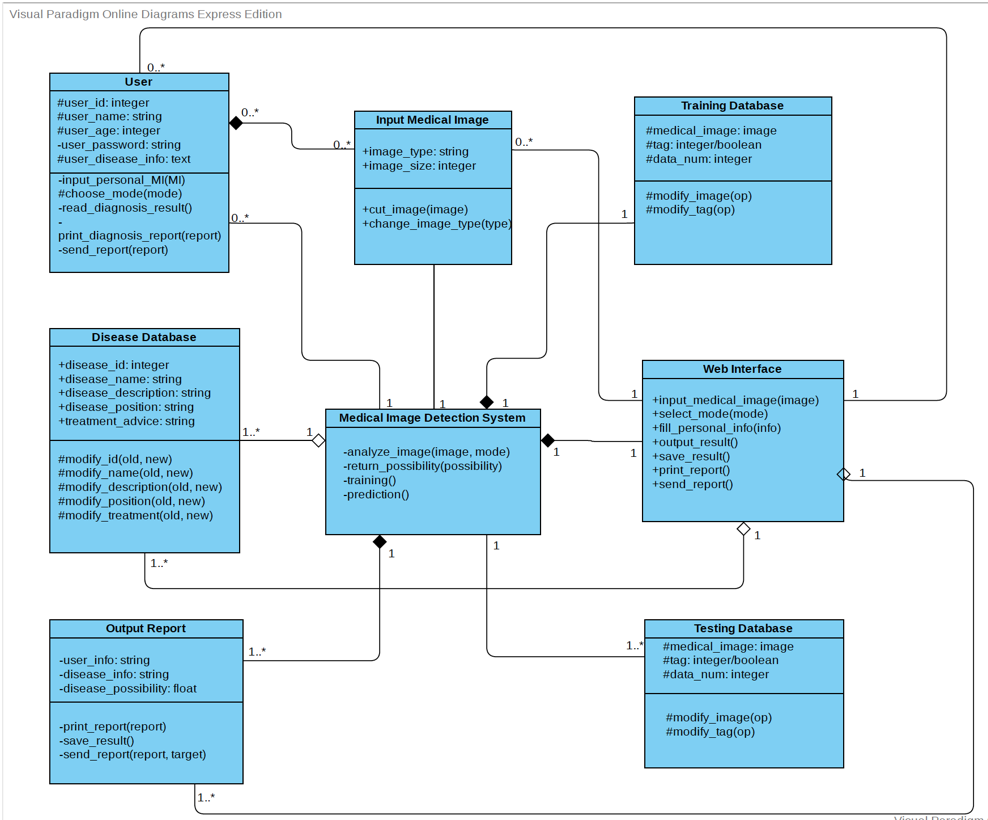
\includegraphics[width=0.9\textwidth]{figures/class}
  	\caption{Class Diagram for Medical Bot System Baseline Situation}
  	\label{fig:class-diagram}
  \end{figure}

  \begin{figure}[H]
	\centering
	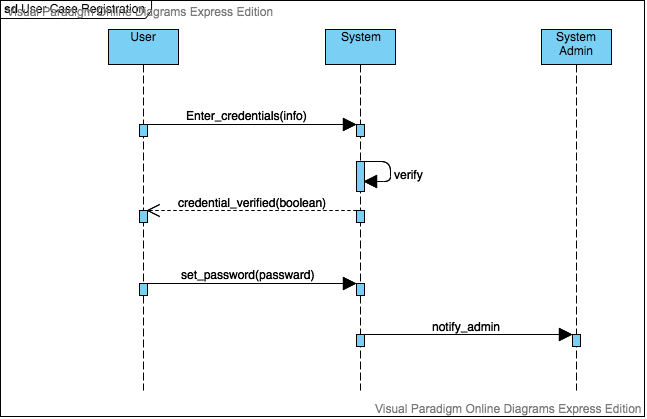
\includegraphics[width=0.9\textwidth]{figures/registration}
	\caption{Sequence Diagram for User Case One - Registration}
	\label{fig:registration}
  \end{figure}

  \begin{figure}[H]
	\centering
	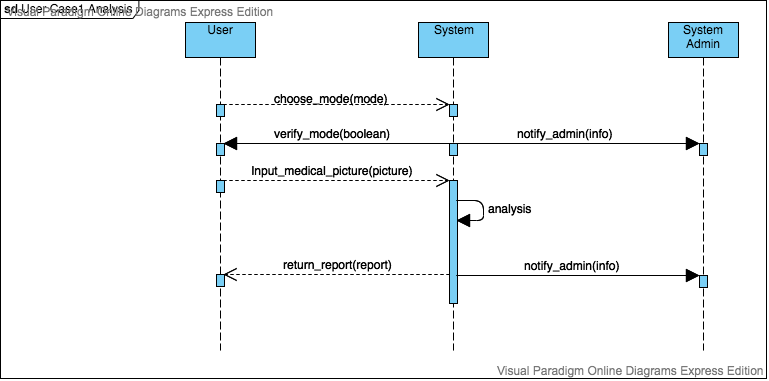
\includegraphics[width=0.9\textwidth]{figures/image-analysis}
	\caption{Sequence Diagram for User Case Two - Medical Image Analysis}
	\label{fig:image-analysis}
  \end{figure}

  \begin{figure}[H]
  	\centering
  	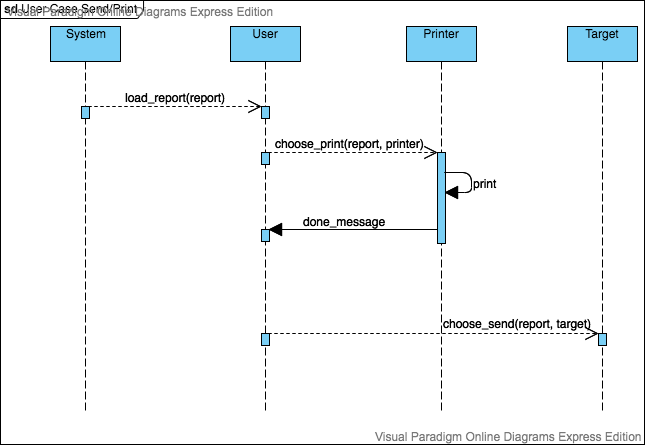
\includegraphics[width=0.9\textwidth]{figures/send}
  	\caption{Sequence Diagram for User Case Three - Send/Print}
  	\label{fig:send}
  \end{figure}
  
  
  \subsection{Implementation Strategies}
  
  \subsubsection{Development Model}
  
  The software process is determined to be combined of two approaches: plan-driven process and agile process.
  
  The plan-driven process will be applied for baseline implementation: Pulmonary Nodules Detection Software, considering the writers have a complete and intact idea of frame, structure and prospective functions for this baseline, which has been described detailedly in the system design part. The waterfall model is used with five stages: requirement definition, system and software design, implementation and unit testing, integration and system testing and operation and maintenance, and each stage is explicitly described in the proposal.
  
  The agile process will mainly be used for further implementation after realizing the baseline, considering optimizing the system would be relatively flexible and planning is incremental, it is easier to change the process and detailed functions with market’s inconstant requirements. Integration and configuration model is more suitable for this project: systems integrated from existing components or COTS systems of different CAD (Computer Aid Diagnosis) fields and mature algorithms will be taken as reused elements, which, despite the baseline Pulmonary Nodule Detection system, will include but not limited to Artificial Intelligent ChatBot for disease consultation, Risk assessment of Alzheimer's disease by detecting retina neural, Stroke risk assessment from brain CT/MRI medical images.
  
  
  
  \subsubsection{Dataset preprocessing}
  
  We plan to preprocess the data using Python and its third-part library Numpy. A series of operations would be applied upon the submitted medical image, including the following:
  \begin{enumerate}
  	\item Convert the input image, which is supposed to be of type CT, to .raw or .mhd format;
  	\item Denoising, coordinate transformation, resolution unification, etc;
  	\item   3D-patching, hard sample mining, data augmentation, etc.
  \end{enumerate}
  For dataset, we plan to train our model on LUNA, which is a frequently used benchmark in the pneumonia diagnosis community.
  
  
  \subsubsection{Ml model training \& prediction}
  We will build our machine learning model using Pytorch in Python, because Pytorch is exactly the appropriate framework for structuring a small-scaled model, and it can fully make use of the speed-up of GPU to accelerate the computation so as to achieve better online interactive results. For pneumonia, the proposed model will mainly contain two parts, the first one of which is responsible for body part detection, while the second part takes as input the outputs of the first part and deals with the classification problem to decide whether the submitted image implies illness. 
  
  Based on the well-defined model, we will train and test it using cross-validation strategy, until it converges. This provides a set of optimal parameters which can be directly used for the real-time, online diagnosis.  
  
  
  \subsubsection{Website development}
  
  The expected product we hope to achieve is a web-based software. For the front end, we plan to use css, HTML, and Javascript to build up the web-page. Node-js will be utilized for the service end. In order to build the backend database of the images, we plan to use MongoDB in Python. 
  
  \subsection{Possible Advanced Development}
  
  \subsubsection{ChatBot}
  
  An advanced version of our project may additionally contain a ChatBot. Two types of ChatBot may be implemented, with one facing the patients and the other one mainly being functional to the doctors. After acquiring the test results from the model, the patient can obtain some supplementary information by using the ChatBot. For instance, when the patient enters symptom description, the ChatBot may grasp the key words and provide some possible curing measures. As for the doctors, the ChatBot may be used as an encyclopedic reference, where they can obtain comprehensive information about the disease of interest. 
  
  \subsubsection{Test for more types of disease}
  
  Apart from pneumonia, there are numerous kinds of diseases where computer vision techniques may also be instrumental. Alzheimer is a typical example of such malady where scientists have paid much efforts. Based on such consideration, it would be of great benefit if we can augment the functionality of our model, so that the input covers a wider range of medical image types, and a more diverse variety of diseases can be automatically diagnosed by utilizing our model. Considering that Numpy alone may not be sufficient for data preprocessing when more diseases are accounted, we would also exploit Pandas and some other libraries when necessary. 
  
   \begin{figure}[H]
  	\centering
  	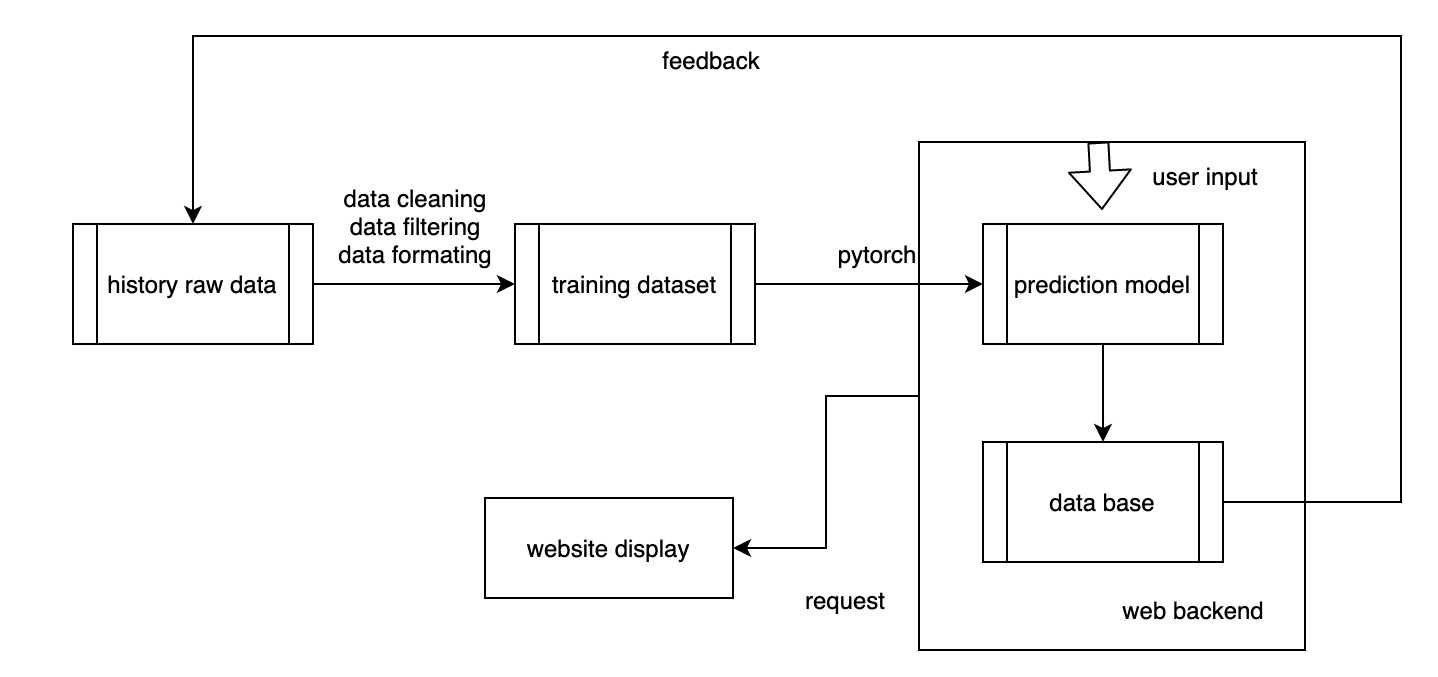
\includegraphics[width=0.9\textwidth]{figures/flow}
  	\caption{Data flow of the expected system (including the advanced functions)}
  	\label{fig:flow}
  \end{figure}
  
  \begin{figure}[H]
  	\centering
  	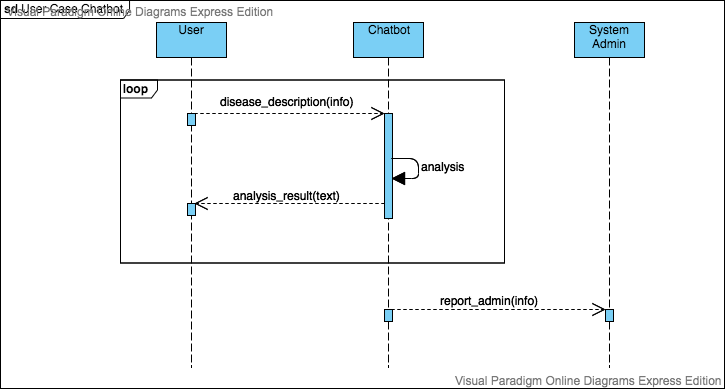
\includegraphics[width=0.9\textwidth]{figures/chatbot}
  	\caption{Sequence Diagram for User Case Four - Chatbot}
  	\label{fig:chatbot}
  \end{figure}

	\begin{figure}[H]
		\centering
		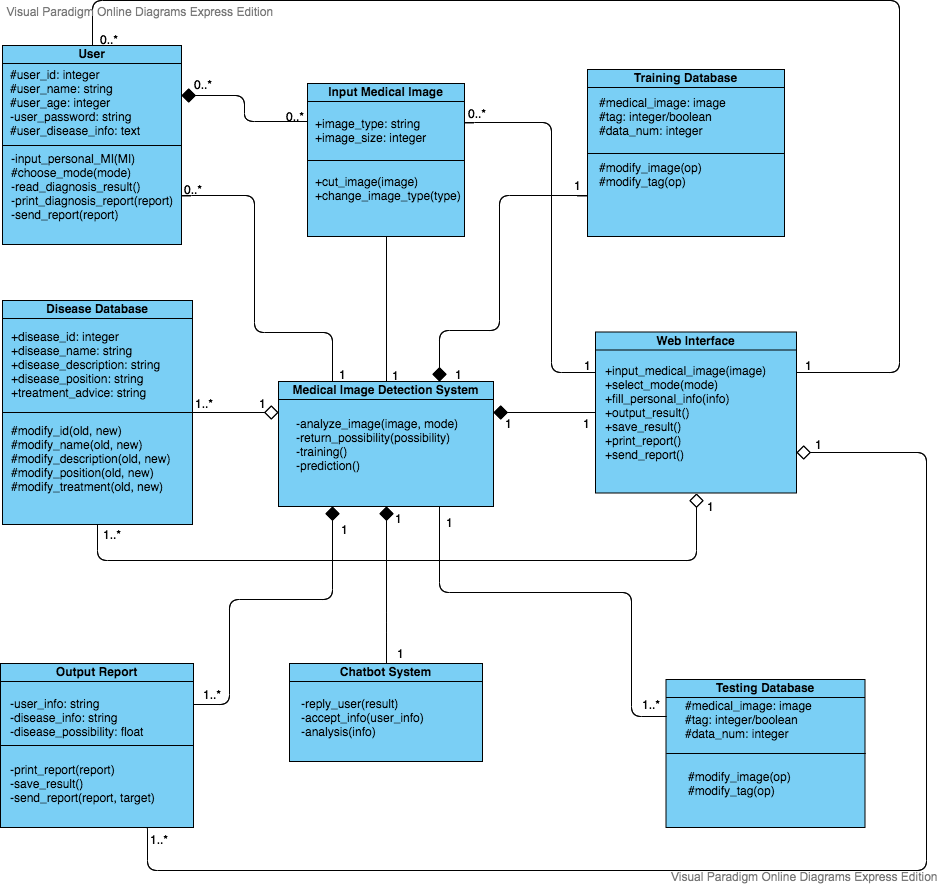
\includegraphics[width=0.9\textwidth]{figures/class-with-chatbot}
		\caption{Class Diagram for Medical Bot System with the Advanced Functionsn}
		\label{fig:class-with-chatbot}
	\end{figure}
  
  \section{Software Testing}
  
  \subsection{Test Planning}
  The objective of the test is to verify that the functionality of the Web-based Medical Bot works as the specifications are intended. Our test programs will execute and verify the test scripts,  identifying errors, anomalies, undesirable features, or information about the software's non-functional attributes.
  
  The final products of the test are the following two:
  \begin{itemize}
  	\item A production-ready software;
  	\item A set of reliable test scripts that can be reused for Unit and Functional test execution.
  \end{itemize}

	Figure \eqref{fig:testing} shows the model of the testing process \footnote{From textbook Fig 8.3}.
	
	\begin{figure}[H]
		\centering
		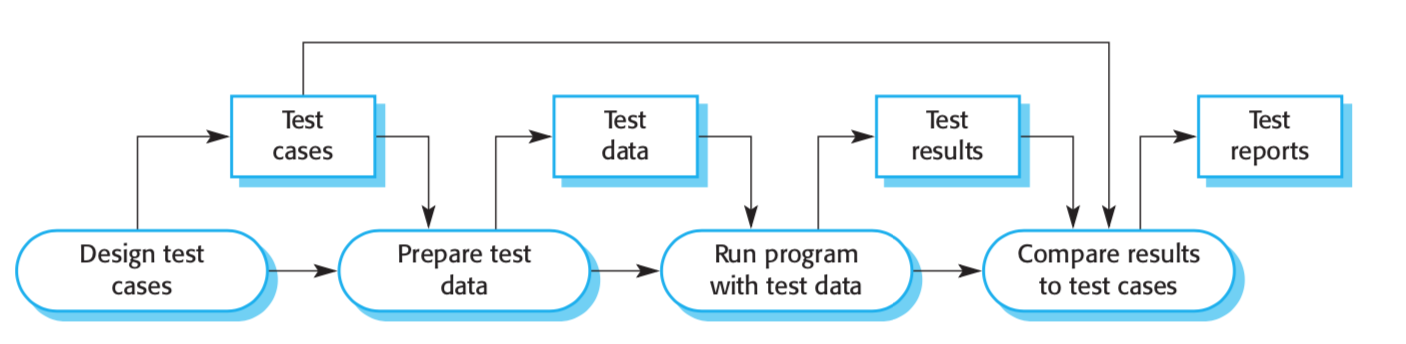
\includegraphics[width=0.9\textwidth]{figures/testing}
		\caption{A model of the software testing process}
		\label{fig:testing}
	\end{figure}
  
  \subsubsection{Test Assumptions}
  
  \begin{itemize}
  	\item Pre-processed medical data required are available in the system prior to the start of ML model training.
  	\item Performance Testing is considered for ML model training.
  	\item Test environment will be set up in all team member's laptops.
  	\item Team members will be paired up to review all the test deliverables.
  	\item The system will be tested as a black box; if the information shows correctly online and in the reports, it will be assumed that the trained models are working properly.
  \end{itemize}
  
  \subsection{Test Design}
  
  \subsubsection{Development Testing}
  We will be carrying out the following three stages of testing
  \begin{enumerate}
  	\item \emph{Unit testing}: Unit tests will be carried out with the development of the software against individual function units or object classes to ensure every core functions' full functionality. Example: use prepared test data as input to see if the predict() function outputs valid results; input an image to check if function \texttt{read\_image()/save\_image()} reads/saves the image as intended;
  	
  	\item \emph{Component testing}: Tests against composite components comprising a group of individual units. Example: check camera component as a whole to see if it’s allowing people to take/upload medical images; check result-displaying component on the front end if it’s functioning as intended; object interfaces validation;
  	
  	\item \emph{System testing}: All components are integrated and the system is tested as a whole. The test focuses on validating the interactions between the components and objects, and cased-based tests will be utilized. Example: test reusable components to check that they work as expected when they are integrated with new components; walk through the process view diagrams (Figures \eqref{fig:registration}, \eqref{fig:image-analysis} and \eqref{fig:send}) and check the responses.
  	
  \end{enumerate}
  
  \subsubsection{Release testing}
  
  We will test if our software meets all the requirements in this step. We are to develop several related tests:
  
  \begin{enumerate}
  	\item Set up a patient account with no medical record. Log in. Upload photos, get a diagnosis report, and prescribe to doctoral suggestions if any.
  	\item Set up a patient account with medical records. Log in. Upload photos, get a diagnosis report, and prescribe to doctoral suggestions. 
  \end{enumerate}
  
  \subsubsection{User testing}
  
  We will be doing a \emph{Beta testing}, where a release of the software is made available to a group of users to allow them to experiment and to raise problems that they discover with the system developers.
  
  \subsection{Test Execution}
  
  Tests will be developed incrementally as the project is developing, and we will run regression tests to check that changes to the project have not introduced new bugs. 
  
  \section{Work Division}
  
  \subsection{Labor Division}
  
  \begin{itemize}
  	\item Implementation of CV and ML algorithms
  	\item Data processing
  	\item Model training and testing
  	\item Web development
  	\item Chatbot development
  \end{itemize}
  
  \subsection{Timeline}
  
  \begin{table}[H]
  	\centering
  	\small
  	\vspace{5pt}
  	\begin{tabular}{p{2cm}p{4.1cm}p{2.4cm}p{4cm}p{2.3cm}}
  		\toprule
  		\textbf{Date} & \textbf{Activity 1} & \textbf{Member} & \textbf{Activity 2} & \textbf{Member}\\
  		\midrule
  		- March 14 & \tabincell{l}{1. Determine the project\\ topic\\
  				2. Literature review\\
  				3. Determine the applica-\\tion requirement\\
  				4. Determine the machine\\ learning model}
  	& \tabincell{l}{Zheyuan Zhou\\
  		Jiazhen Liu\\
  		Chunyue Xue\\
  		Shiting Xiao\\
  		Yaqian Chen
  	} & & \\ \hline
  	 
  		March 14 - 21 & \tabincell{l}{1. Write the midterm pro-\\posal\\
  			2. Prepare computer en-\\vironment\\
  			3. Determine the ML algo-\\rithm and web framework}
  		& \tabincell{l}{Zheyuan Zhou\\
  			Jiazhen Liu\\
  			Chunyue Xue\\
  			Shiting Xiao\\
  			Yaqian Chen
  		} & &  \\ \hline
  	
  	March 21 - 29 &\tabincell{l}{Integrate the proposal\\ components and slight\\ modification} 
  	& \tabincell{l}{Zheyuan Zhou\\
  		Jiazhen Liu\\
  		Chunyue Xue\\
  		Shiting Xiao\\
  		Yaqian Chen
  	} & &\\\hline
  
  	  March 29 - April 5 & \tabincell{l}{Learn the basic CV and\\ ML algorithm}
  	  & \tabincell{l}{
  	  	Jiazhen Liu\\
  	  	Chunyue Xue\\
  	  	Shiting Xiao
  	  } & 
    \tabincell{l}{Learn the basic web\\implementation} 
    & \tabincell{l}{
    	Zheyuan Zhou\\
    	Yaqian Chen
    }  \\\hline
	
	April 5 - 26 & \tabincell{l}{Develop the prediction\\ model (including data pre-\\processing, training and \\testing) for basic applica-\\tion requirement (Tumor\\recognition and initial di-\\agnosis)}
	& \tabincell{l}{
		Jiazhen Liu\\
		Chunyue Xue\\
		Shiting Xiao
	} & 
	\tabincell{l}{Develop the website in-\\cluding database, web in-\\terface, web frontend for\\ basic application require-\\ment (Tumor recognition \\and initial diagnosis)}
	& \tabincell{l}{
		Zheyuan Zhou\\
		Yaqian Chen
	}  \\\hline
	
	April 26 - May 3 &\tabincell{l}{Test the basic web func-\\tions and conduct slight \\modification} 
	& \tabincell{l}{Zheyuan Zhou\\
		Jiazhen Liu\\
		Chunyue Xue\\
		Shiting Xiao\\
		Yaqian Chen
	} & &\\\hline

	May 3 - 10 & \tabincell{l}{1. Search the relative psy-\\chology information for\\ real-time monitoring of \\patients' mental health\\
		2. Develop the online re-\\gistration function}
	& \tabincell{l}{
		Jiazhen Liu\\
		Chunyue Xue\\
		Shiting Xiao
	} & 
	\tabincell{l}{1. Develop the ChatBot \\function for patients to \\directly consult doctors\\
		2. Include the consulting\\ room function based on\\ LAN which supports the\\ online consulting}
	& \tabincell{l}{
		Zheyuan Zhou\\
		Yaqian Chen
	}  \\
  		\bottomrule
  	\end{tabular}
    \caption{Timeline for the development process}
  \end{table}

\newpage
\bibliography{proposal}{}
\bibliographystyle{plain}
  
\end{document}